\subsection{Company Structure}

Company structure is shown in Figure \ref{fig:company_structure}.

\begin{figure}[h]
    \centering
    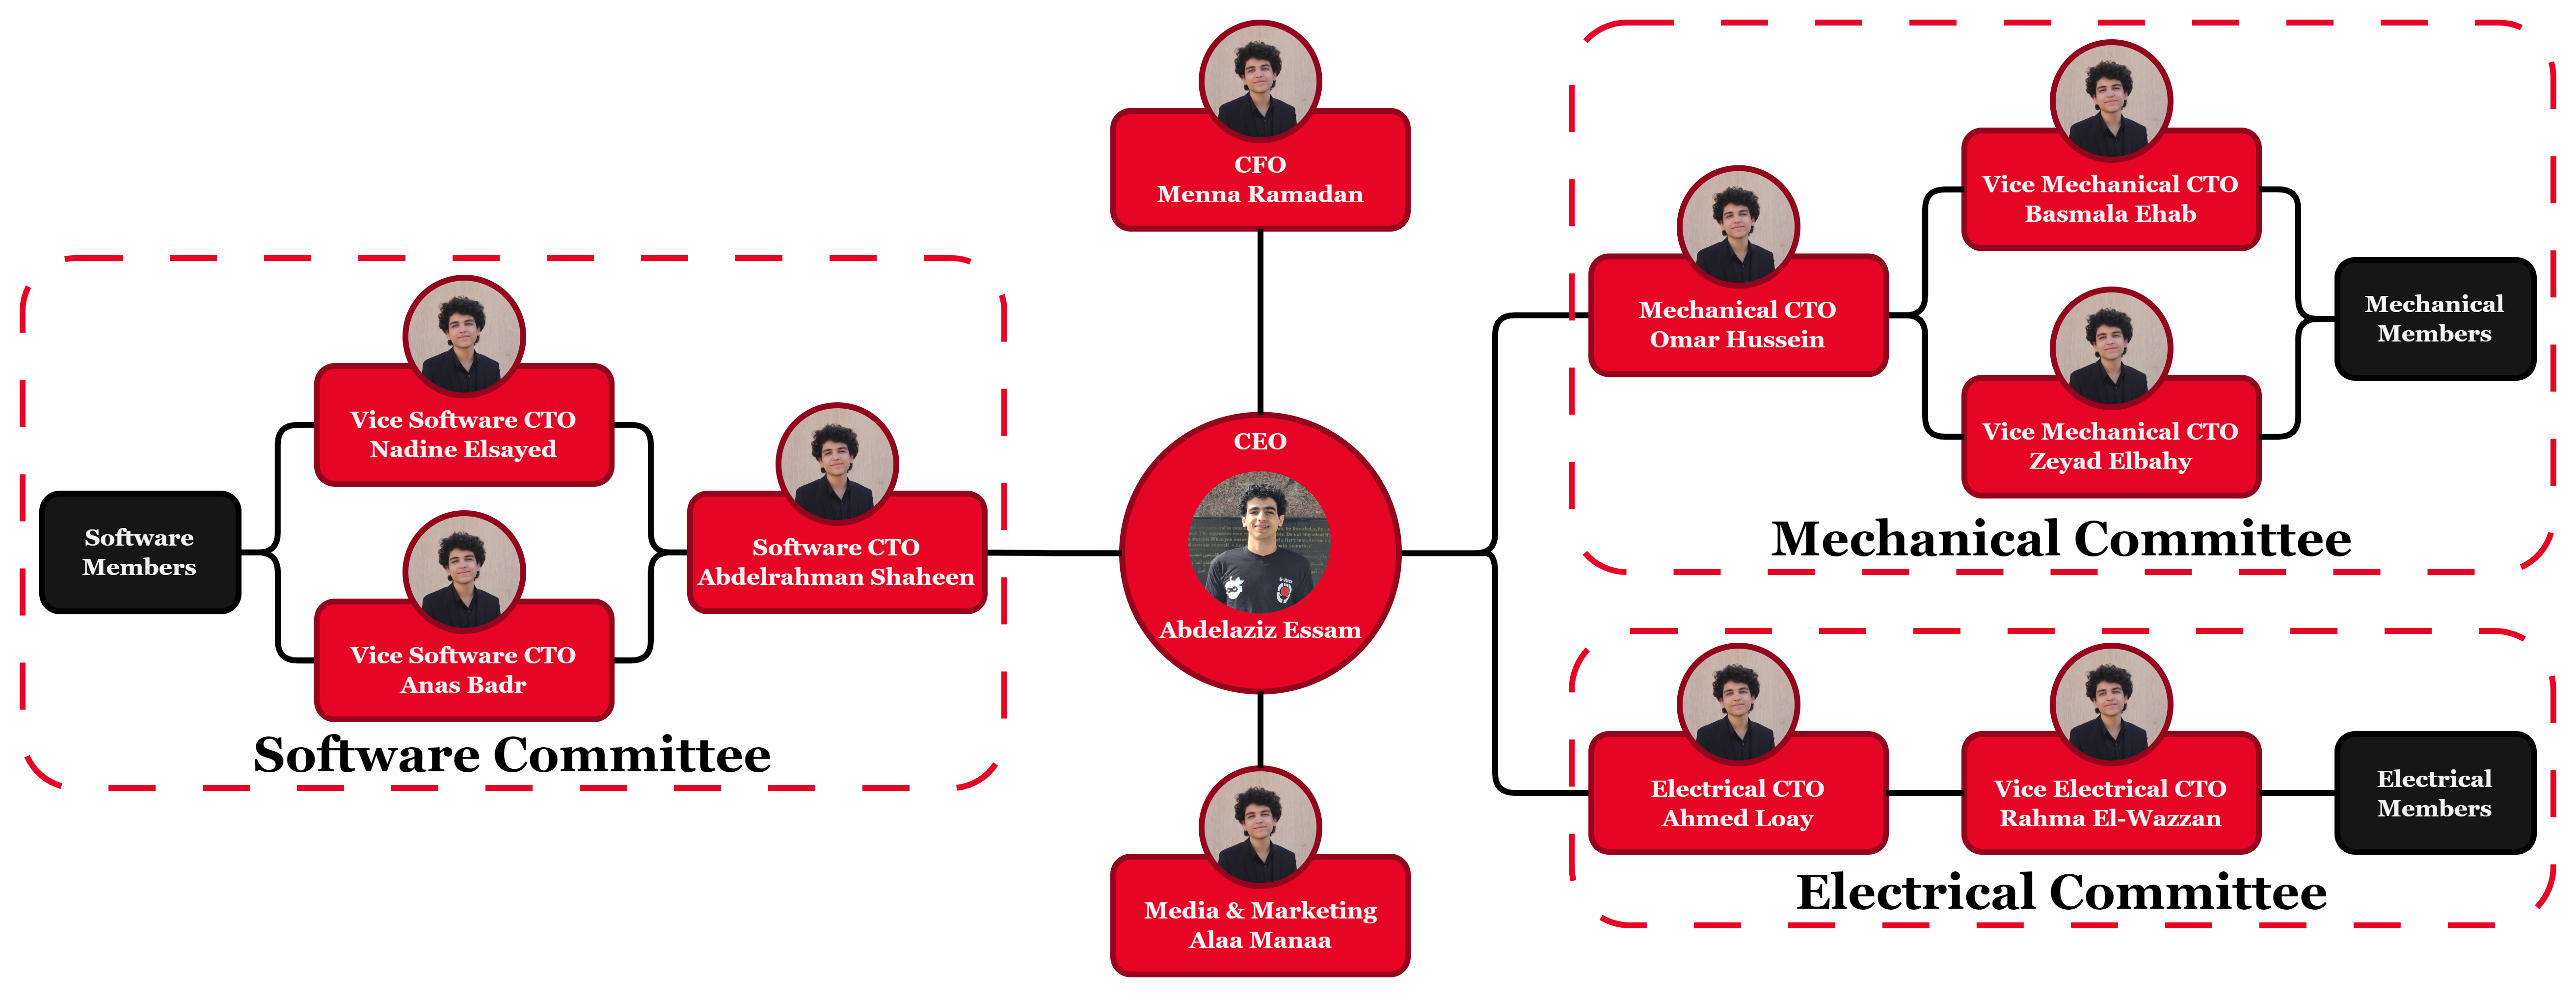
\includegraphics[width=\columnwidth]{Sections/5Logistics/images/ROV hierarchy.png}
    \caption{Company Structure.}
    \label{fig:company_structure}
\end{figure}

\textbf{Team Board}
\vspace{-0.5\baselineskip}
\begin{itemize}[leftmargin=0pt, itemindent=20pt]
    \setlength{\itemsep}{0pt}
    \item \textbf{CEO (Chief Executive Officer):} Oversees all activities and high-level decision-making.
    \item \textbf{CFO (Chief Financial Officer):} Manages budget, funding, and financial operations.
\end{itemize}

\textbf{Technical Sector}

The technical sector has three divisions, each led by a CTO (Chief Technical Officer) and Vice CTOs:
\vspace{-0.5\baselineskip}
\begin{enumerate}[leftmargin=0pt, itemindent=20pt]
    \setlength{\itemsep}{0pt}
    \item \textbf{Mechanical Committee:} Responsible for designing and manufacturing the physical structure of Kamikaze.
    \item \textbf{Electrical Committee:} Develops and integrates power distribution and control systems.
    \item \textbf{Software Committee:} Focuses on control algorithms, vision processing, and system automation.
\end{enumerate}

\textbf{Non-Technical Sector}

Beyond technical development, the Non-Technical Team plays a key role in logistics, outreach, and team operations:
\vspace{-0.5\baselineskip}
\begin{itemize}[leftmargin=0pt, itemindent=20pt]
    \setlength{\itemsep}{0pt}
    \item \textbf{Logistics:} Plans events and coordinates resources.
    \item \textbf{PR:} Manages communications and partnerships.
    \item \textbf{Media \& Marketing:} Creates content and manages social media.
    \item \textbf{Sponsorship \& Fundraising:} Secures funding and sponsors.
    \item \textbf{Event Management:} Organizes workshops and outreach.
\end{itemize}
